% !TeX program = pdflatex
% This editable project is generated from the canonical Markdown manuscript.
% Preserve the supervisor's chinese.cls, with numbered references for the existing bibliography.
\documentclass[numdoi]{chinese}
\usepackage{booktabs,longtable,array,caption}
\usepackage{xurl}
\usepackage[unicode,hidelinks]{hyperref}
% Restrict the legacy CJK Unicode maps to CJK fonts so Latin text remains searchable.
\makeatletter
\let\gmOriginalCJKAddCmap\CJK@addcmap
\def\CJK@addcmap#1{%
  \edef\gmCJKEncoding{C70}%
  \ifx\f@encoding\gmCJKEncoding\gmOriginalCJKAddCmap{#1}\fi}
\makeatother
\urlstyle{same}
% Keep the original manuscript spacing; dense tables and captions remain single-spaced.
\pagestyle{plain}
\setlength{\emergencystretch}{2em}
\captionsetup{font={small,stretch=1},justification=justified,singlelinecheck=false,skip=5pt}
\newlength{\gmTableWidth}
% Use the Chinese bibliography heading while retaining the template's numbered reference layout.
\renewcommand{\refname}{参考文献}
\setcounter{topnumber}{3}
\renewcommand{\topfraction}{0.95}
\renewcommand{\textfraction}{0.03}
\renewcommand{\floatpagefraction}{0.75}
\hypersetup{pdftitle={面向地球系统模式的全球网格数据库：GriddingMachine框架更新与应用},pdfauthor={Hao Jiang; Yujie Wang}}
\begin{document}
\doublespacing
\begin{CJK}{UTF8}{gbsn}

% Preserve the supplied title block and the confirmed two-author list.
{\centering
\par\noindent {\Large\textbf{面向地球系统模式的全球网格数据库：GriddingMachine框架更新与应用}\par}
\normalsize
\par\noindent \textbf{姜皓}\textsuperscript{1,2}　\textbf{王玉杰}\textsuperscript{1,2,*}
\par\noindent \textsuperscript{1} 中国科学技术大学风云卫星遥感联合实验室
\par\noindent \textsuperscript{2} 崂山实验室
\par\noindent \textsuperscript{*} 通讯作者（wyujie@ustc.edu.cn）
\par}
\section*{摘要}
地球系统模式依赖区域至全球尺度的网格数据进行参数初始化及结果验证。尽管当前数据大多已采用NetCDF、\allowbreak{}HDF、\allowbreak{}GeoTIFF等标准格式，不同数据源在处理规则、\allowbreak{}单位、\allowbreak{}数据标识和网络分发方式等方面仍存在差异，研究人员往往需要针对各自模式重复整理和维护数据库，增加了模式持续更新与验证的工作量。本文在2022版GriddingMachine基础上，围绕数据预处理、\allowbreak{}分发和读取进行改进。通过共享配置统一组织数据处理规则，使不同来源的数据能够按一致规范完成标准化；采用直接NetCDF分发和独立维护的数据目录，简化数据获取与更新；进一步将多源数据组织为陆面参数和气象驱动，为模式计算提供输入。应用案例表明，改进后的流程能够保持标准化结果与独立参考的一致性，缩短数据获取至首次读取的时间，并在数据修订后沿用已有标签访问，支持多源数据向模式输入的衔接。此外，完善了Matlab、\allowbreak{}Octave、\allowbreak{}Python和R语言对新版数据的自动下载支持，并新增C和Fortran语言的自动下载支持，以更好地服务科学研究与应用。

\textbf{关键词：} 地球系统模式；全球网格数据库；数据标准化；NetCDF；数据完整性；模式输入

\begin{center}\large \textbf{A Global Gridded Database for Earth System Models: Advances and Applications of GriddingMachine}\end{center}
\begin{center}\small \textbf{Hao JIANG}\textsuperscript{1,2}, \textbf{Yujie WANG}\textsuperscript{1,2,*}\end{center}
\begin{center}\small \textsuperscript{1} Joint Laboratory of Fengyun Remote Sensing, University of Science and Technology of China\end{center}
\begin{center}\small \textsuperscript{2} Laoshan Laboratory\end{center}
\begin{center}\small \textsuperscript{*} Corresponding author (wyujie@ustc.edu.cn)\end{center}
\section*{Abstract}
Earth system models rely on gridded data at regional to global scales for parameter initialization and evaluation of simulation results. Although most datasets are available in standard formats such as NetCDF, HDF, and GeoTIFF, data sources still differ in processing rules, units, data identifiers, and distribution methods. Researchers therefore often need to organize and maintain databases for individual models, adding to the work required for continued model development and evaluation. Building on the 2022 release of GriddingMachine, this study improves data preprocessing, distribution, and reading. Shared configurations organize processing rules so that data from different sources can be standardized according to common conventions. Direct NetCDF distribution and an independently maintained catalog simplify data acquisition and updates, while land parameters and meteorological forcing are assembled from multiple sources to provide model inputs. Application cases show that the improved workflow maintains agreement between standardized results and independent references, shortens the time from data acquisition to the first read, preserves access through existing labels after data revisions, and connects data from multiple sources to model inputs. Automatic downloading of the updated data has also been improved for MATLAB, Octave, Python, and R, with new support for C and Fortran, to better serve scientific research and applications.

\textbf{Keywords:} Earth system models; global gridded database; data standardization; NetCDF; data integrity; model input

\section{引言}
地球系统模式的参数初始化、\allowbreak{}边界条件、\allowbreak{}气象驱动和结果验证均依赖区域至全球尺度的网格数据。这些数据由不同研究团队和业务机构提供，即使采用相同的文件格式，其坐标排列、\allowbreak{}空间与时间分辨率、\allowbreak{}变量含义、\allowbreak{}单位和缺失值表示仍可能存在差异。研究人员因此需要在数据获取后继续完成转换和整理。此类工作往往随各模式的需求分别开展，源数据或模式接口更新后，相应程序和输入文件还需持续维护。减少同类数据的重复整理，并在更新中保持输入一致，是全球网格数据应用中的实际问题。

科学数据复用需要明确数据的发现、\allowbreak{}访问和解释方式。FAIR原则强调可发现（\textbf{F}indable）、\allowbreak{}可获取（\textbf{A}ccessible）、\allowbreak{}可互操作（\textbf{I}nteroperable）和可复用（\textbf{R}eusable）\cite{ref1}；NetCDF及气候与预报元数据约定（Climate and Forecast Metadata Conventions，CF）为多维数据、\allowbreak{}坐标和变量属性的表达提供基础\cite{ref2,ref3}。Google Earth Engine等云平台通过改善数据表达、\allowbreak{}发现、\allowbreak{}访问及计算，提升了大尺度地学数据的访问和分析能力\cite{ref4}。本地模式试验还需保存可反复调用的处理结果，并记录所用数据版本和转换规则。对于面向固定版本、\allowbreak{}离线缓存和模式直接调用的工作流，研究人员仍需要把数据转换规则、\allowbreak{}标准数据标识、\allowbreak{}网络获取内容和下游模式接口连接起来。因此，建立适用于本地运行的标准化科研数据库，可以集中维护多源数据及其处理结果，为不同模式试验提供一致的数据输入。

Wang等\cite{ref5}于2022年发布了基于Julia语言的GriddingMachine数据库和软件，将常用于陆面和地球系统模拟的全球数据整理为具有统一空间和变量约定的NetCDF文件，通过数据标签和软件包内的Artifacts.toml目录实现管理与自动下载，并提供Julia、\allowbreak{}Matlab、\allowbreak{}Octave、\allowbreak{}Python和R接口。该版本为多源数据的统一访问奠定了基础。随着数据类型和应用需求扩展，原有流程在数据维护和模式接入方面仍有改进空间。处理规则主要保存在数据源专用脚本中，新增数据需要分别适配；标准NetCDF经外层tar.gz归档后分发，使用前还需解包。Julia包内的数据目录随软件版本更新，新增或修订数据时需同步维护内置目录。获得标准网格数据后，研究人员仍需根据具体模式组合参数和气象序列，并完成时间与单位换算。

针对这些需求，改进应围绕数据转换规则的复用、\allowbreak{}分发信息的独立维护及模式输入的组织展开。源数据特有的转换规则与通用程序分开，可使新增数据沿用已有处理方法；数据目录独立维护并直接分发NetCDF，可减少更新与获取时的附加步骤；在标准网格读取之后统一处理参数组合、\allowbreak{}时间轴和单位关系，则可减少各模式重复编写数据接入程序。标准NetCDF和数据标签为这些环节提供共同约定，使处理结果能够持续用于模式试验。

本文从数据预处理、\allowbreak{}分发与读取三个方面更新2022版GriddingMachine，通过共享处理规则和独立维护数据目录减少重复整理，并在统一读取基础上组织模式输入。同时完善Matlab、\allowbreak{}Octave、\allowbreak{}Python和R对新版数据的自动下载支持，新增C和Fortran自动下载支持。研究采用受控处理实例和真实海表温度数据检验标准化结果，以高程与叶面积指数数据比较分发效率，并通过网络镜像获取核对文件内容的一致性；最后以Emerald陆面过程模式为例，考察陆面参数与逐时气象数据如何形成模式输入。

\section{框架设计与关键方法}
\subsection{总体架构与数据流程}
新版GriddingMachine按数据处理、\allowbreak{}分发和模式应用的职责划分为三个相互衔接的功能层（图1）。数据生产与标准化层根据源数据和文本配置格式YAML记录的处理规则，完成维度、\allowbreak{}坐标与数值转换，经质量检查后输出标准NetCDF文件。数据目录与可信分发层登记数据标签、\allowbreak{}版本、\allowbreak{}镜像和完整性信息，负责目录更新、\allowbreak{}文件下载与内容核验。模式输入组织层读取已获取的标准化数据，提取目标格点，融合陆面参数并组织气象驱动。数据生产主要由GriddingMachineDatasets承担，目录管理、\allowbreak{}文件获取和模式输入组织主要由GriddingMachine.jl承担。

\begin{figure}[!htbp]
\centering
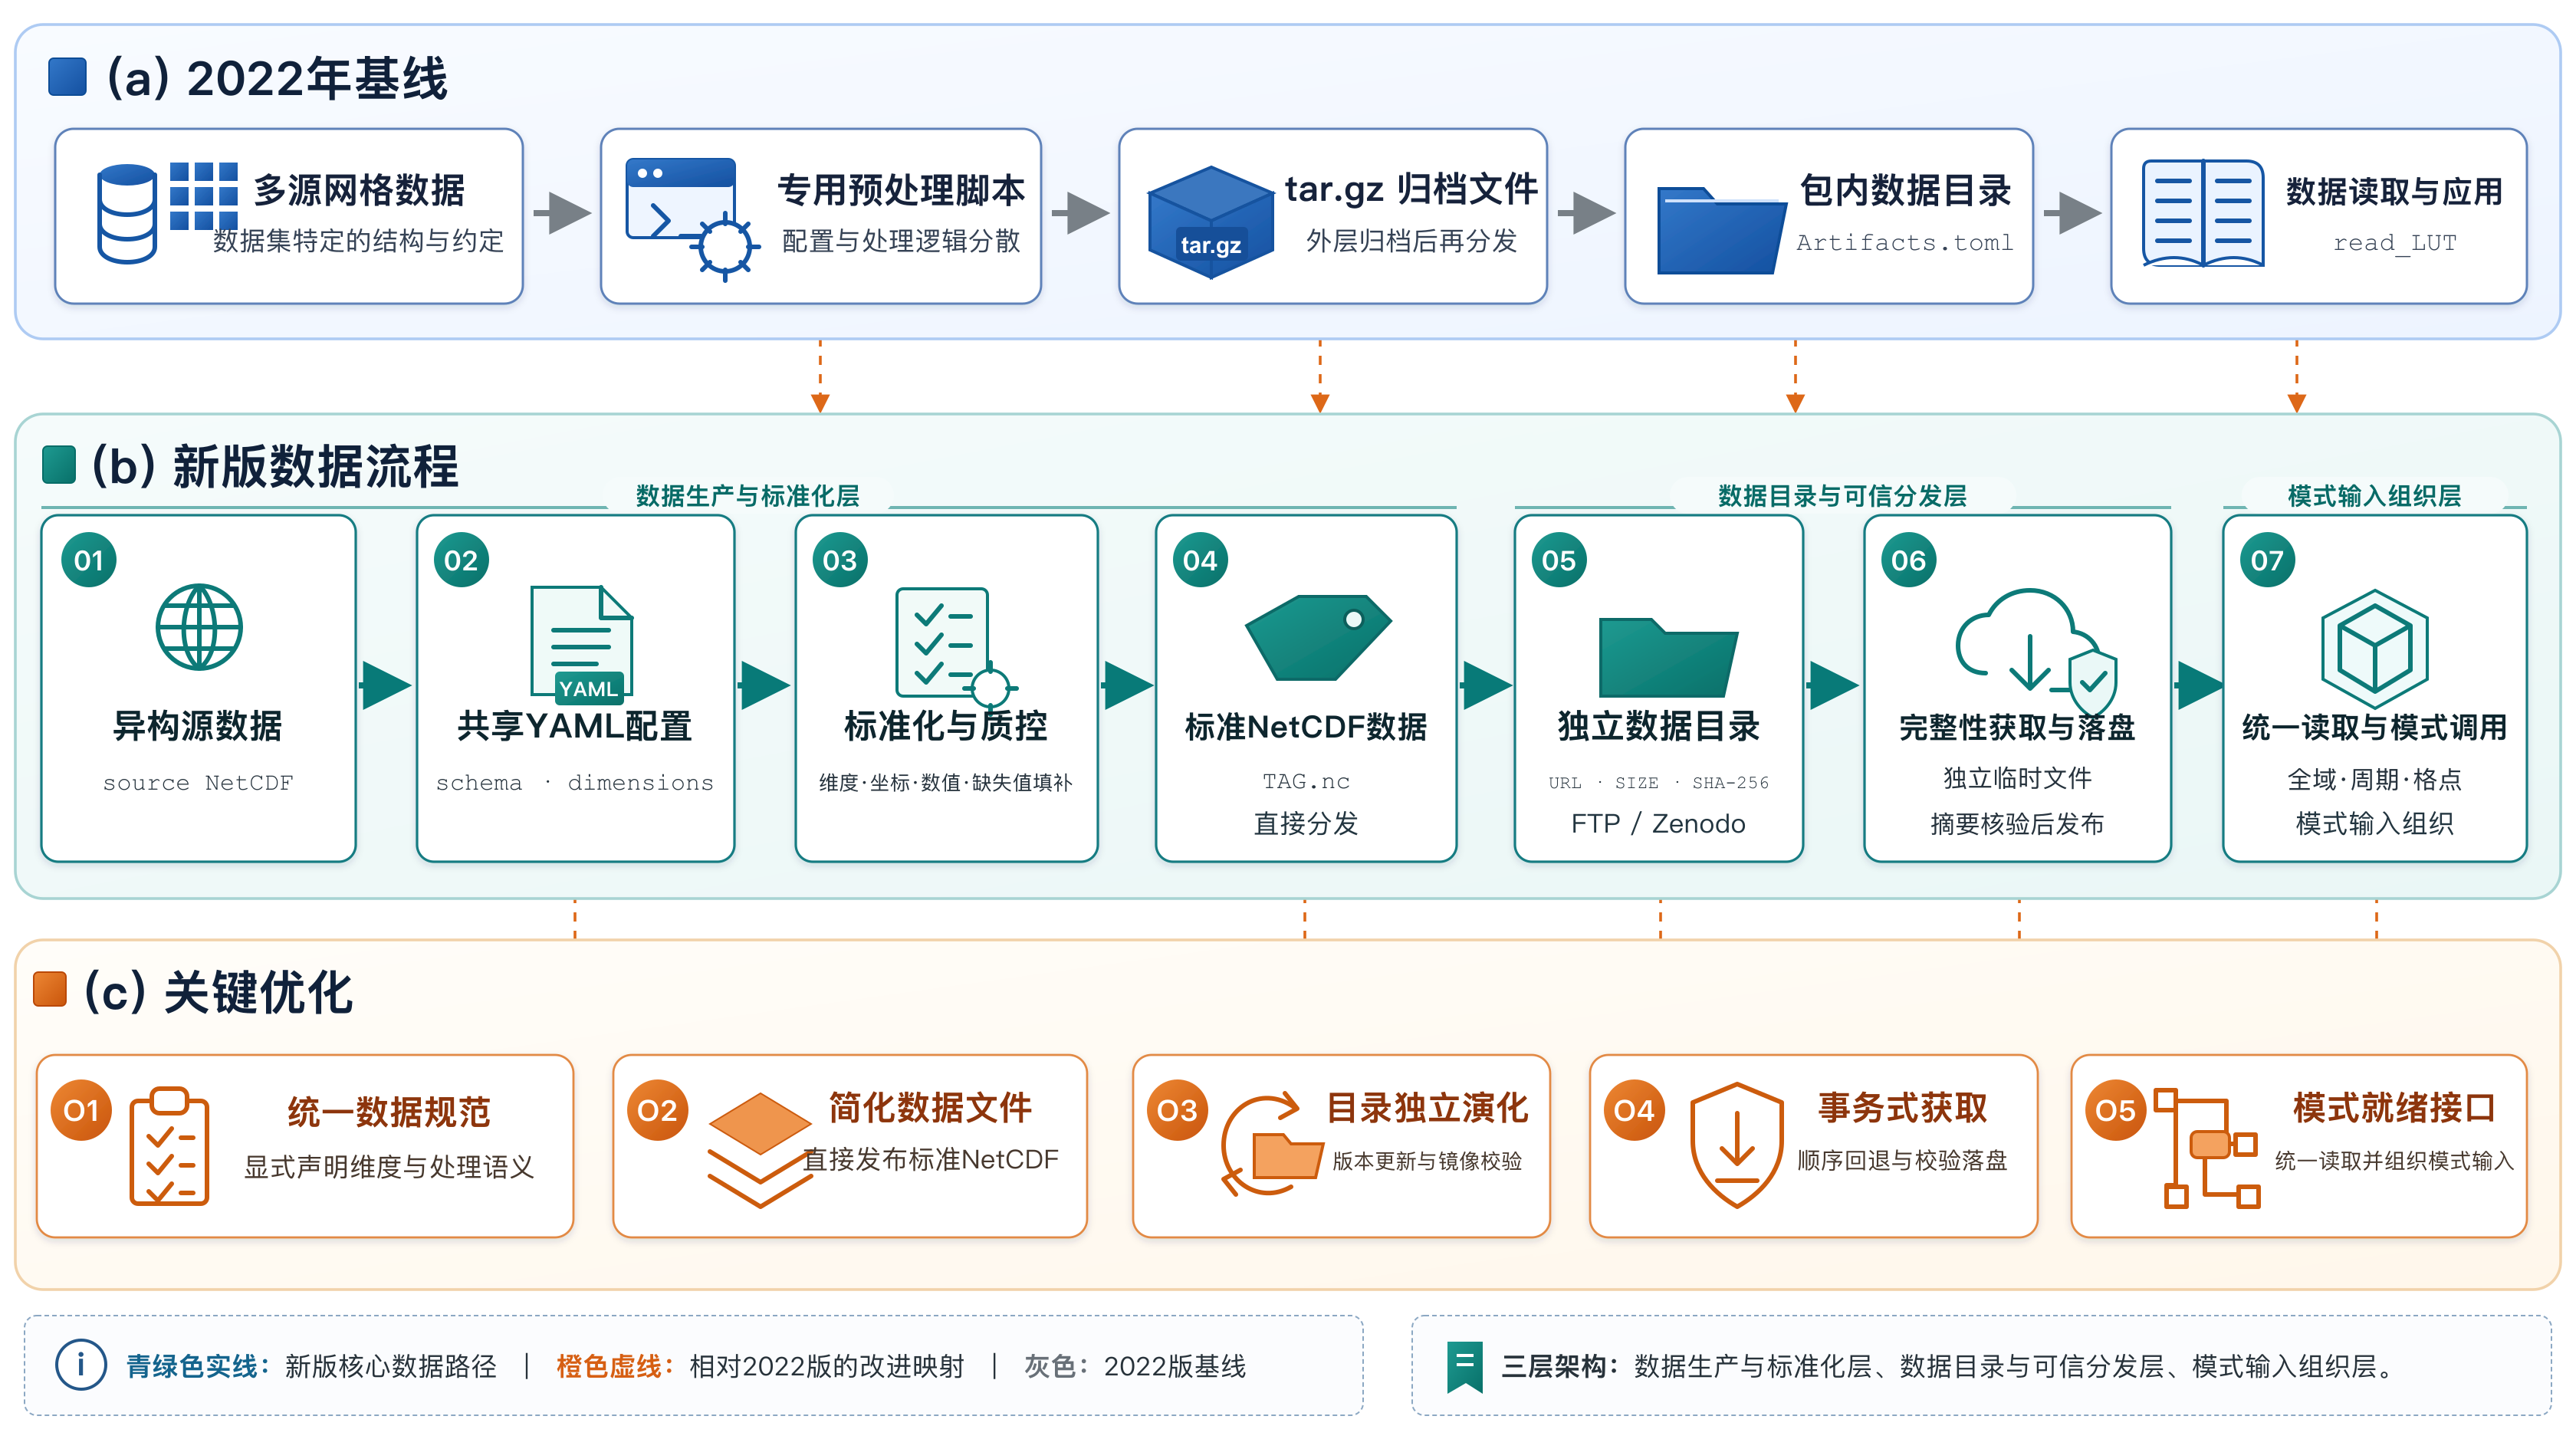
\includegraphics[width=\linewidth,height=0.46\textheight,keepaspectratio]{figures/figure1.png}
\caption*{\textbf{图1 GriddingMachine从2022版基线到新版数据流程的架构更新} （a）2022版以数据集专用脚本、\allowbreak{}\nolinkurl{tar.gz}文件、\allowbreak{}包内数据目录和读取函数\nolinkurl{read_LUT}构成数据预处理、\allowbreak{}分发与读取路径；（b）新版由数据生产与标准化层、\allowbreak{}数据目录与可信分发层和模式输入组织层构成，依次连接异构源数据、\allowbreak{}共享YAML配置、\allowbreak{}标准化与质量控制、\allowbreak{}标准NetCDF、\allowbreak{}独立数据目录、\allowbreak{}完整性获取以及统一读取和模式调用；（c）O1—O5依次表示统一数据规范、\allowbreak{}简化数据文件、\allowbreak{}目录独立演化、\allowbreak{}事务式获取和模式就绪接口。橙色虚线标示各项更新相对于2022版基线及新版核心节点的对应关系。}
\caption*{\textbf{Fig. 1 Architectural updates from the 2022 GriddingMachine baseline to the updated data workflow.} (a) The 2022 release linked dataset-specific preprocessing, \nolinkurl{tar.gz} distribution, an in-package catalog, and \nolinkurl{read_LUT}. (b) The updated framework connects configuration-driven standardization, direct NetCDF distribution, an independent catalog with integrity-verified acquisition, and model-input organization. (c) O1--O5 summarize updates to data specifications, file distribution, catalog maintenance, transactional acquisition, and model-ready interfaces. Orange dashed lines link these updates to the corresponding baseline components and updated workflow nodes.}
\label{fig:1}
\end{figure}
三个功能层通过标准NetCDF和数据标签连接。生产流程输出以标签命名的文件，数据目录记录标签对应的文件地址，科研程序据此获取和读取数据。源数据变化时更新处理配置，分发位置变化时调整目录，模式程序则沿用统一读取方式，并根据自身接口组织输入。这样，处理规则、\allowbreak{}分发信息和模式接入程序可以分别维护。具体方法见第2.2—2.4节。

表1对比2022版与新版在数据生产、\allowbreak{}分发、\allowbreak{}读取和跨语言获取方面的主要差异。

% Keep captions and all rows together; thin rules distinguish parallel entries.
\begin{table}[!htbp]\centering
\begingroup\singlespacing\small\setlength{\tabcolsep}{9pt}\renewcommand{\arraystretch}{1.12}
\captionsetup{justification=centering}
\setlength{\gmTableWidth}{\dimexpr\linewidth-4\tabcolsep\relax}
\caption*{\textbf{表1 2022版与新版GriddingMachine的功能和技术路线比较}}
\caption*{\textbf{Table 1 Comparison between the 2022 release and the updated GriddingMachine.}}
\begin{tabular}{@{}>{\raggedright\arraybackslash}p{0.17\gmTableWidth}>{\raggedright\arraybackslash}p{0.36\gmTableWidth}>{\raggedright\arraybackslash}p{0.47\gmTableWidth}@{}}
\toprule
\textbf{更新环节} & \textbf{2022版} & \textbf{新版} \\
\midrule
数据生产 & 数据源专用脚本与贡献流程 & 共享YAML配置、\allowbreak{}源维度映射及配置生成 \\
\midrule[0.25pt]
分发文件 & NetCDF外层\nolinkurl{tar.gz}归档 & 直接分发NetCDF，省去外层解包 \\
\midrule[0.25pt]
目录维护 & Julia包内置\nolinkurl{Artifacts.toml} & 独立\nolinkurl{Artifacts.yaml}，与软件版本分别更新 \\
\midrule[0.25pt]
文件获取 & 多URL下载、\allowbreak{}哈希核验及解包 & 多镜像回退，临时文件核验后更新正式文件 \\
\midrule[0.25pt]
数据读取 & \nolinkurl{read_LUT}提供全域网格、\allowbreak{}周期切片及格点读取 & \nolinkurl{read_dataset}统一读取入口，兼容\nolinkurl{read_LUT} \\
\midrule[0.25pt]
模式输入 & 标准化数据与通用读取 & 陆面参数融合、\allowbreak{}气象驱动组织及Emerald接口 \\
\midrule[0.25pt]
多语言获取 & Julia、\allowbreak{}Matlab、\allowbreak{}Octave、\allowbreak{}Python和R接口 & 完善原有下载支持，新增C和Fortran；各下载入口支持URL、\allowbreak{}标签与完整性核验 \\
\bottomrule
\end{tabular}
\endgroup
\label{tab:1}
\end{table}
研究所用目录版本收录1179个数据条目，包括高程与陆地掩膜、\allowbreak{}土壤水力性质、\allowbreak{}植被结构与叶片属性，以及气象驱动等数据。地形和土壤属性用于描述格点的基础陆面条件，植被数据包含季节变化信息，逐时气象数据提供模式运行的外部驱动。数据标签按类别、\allowbreak{}空间与时间分辨率、\allowbreak{}年份和版本组织；各条目登记机构文件传输协议（File Transfer Protocol，FTP）地址，部分同时配置Zenodo镜像。预定义陆面参数集合将土壤、\allowbreak{}冠层和叶片等数据按字段组合，气象驱动集合则按变量和年份组织逐时数据，便于科研程序按格点与年份获取输入。目录版本与统计记录见补充材料S7。

\subsection{YAML驱动的数据生产与标准化}
\subsubsection{数据规范与维度映射}
GriddingMachine采用NetCDF格式保存多维数组、\allowbreak{}坐标和自描述元数据，便于不同地球科学软件读取\cite{ref2}。2022 年版本已经规定数据采用二维或三维规则经纬网，前两维依次为经度和纬度，可选第三维表示周期；经度自西向东、\allowbreak{}纬度自南向北，输出保存为实际物理值，缺失值在读取后统一表示为 \nolinkurl{NaN}，主变量和不确定性变量分别命名为 \nolinkurl{data} 和 \nolinkurl{std}\cite{ref5}。新版保留这些约定，并进一步规范源维度映射、\allowbreak{}处理记录、\allowbreak{}配置归档和分发完整性信息，使处理程序、\allowbreak{}数据文件和获取接口能够使用同一套规则（表2）。

% Keep captions and all rows together; thin rules distinguish parallel entries.
\begin{table}[!htbp]\centering
\begingroup\singlespacing\small\setlength{\tabcolsep}{9pt}\renewcommand{\arraystretch}{1.12}
\captionsetup{justification=centering}
\setlength{\gmTableWidth}{\dimexpr\linewidth-2\tabcolsep\relax}
\caption*{\textbf{表2 GriddingMachine 标准 NetCDF 数据与元数据规范}}
\caption*{\textbf{Table 2 Standardized NetCDF data and metadata requirements of GriddingMachine.}}
\begin{tabular}{@{}>{\raggedright\arraybackslash}p{0.20\gmTableWidth}>{\raggedright\arraybackslash}p{0.80\gmTableWidth}@{}}
\toprule
\textbf{规范要素} & \textbf{统一约定} \\
\midrule
文件与网格 & 一个标签对应一个NetCDF文件；采用规则经纬网，默认全球覆盖，并声明坐标参考 \\
\midrule[0.25pt]
维度顺序 & 二维\nolinkurl{(lon, lat)}或三维\nolinkurl{(lon, lat, ind)}；源维度按名称映射到标准顺序 \\
\midrule[0.25pt]
坐标方向 & 经度自西向东，范围为\nolinkurl{[-180, 180)}；纬度自南向北；坐标与数据同步变换 \\
\midrule[0.25pt]
数据与元数据 & \nolinkurl{data}为主变量，\nolinkurl{std}为同形不确定性；保存实际物理值、\allowbreak{}变量说明和单位 \\
\midrule[0.25pt]
范围与缺失值 & YAML显式声明有效范围、\allowbreak{}填充值及缺失值处理策略 \\
\midrule[0.25pt]
处理记录 & YAML保存转换规则；输出NetCDF属性记录实际执行的变更 \\
\midrule[0.25pt]
复现信息 & 共同归档配置规范版本（\nolinkurl{SCHEMA_VERSION}）、\allowbreak{}完整YAML、\allowbreak{}固定输入及代码环境 \\
\midrule[0.25pt]
标签与版本 & 标签记录类别、\allowbreak{}空间/时间分辨率、\allowbreak{}年份、\allowbreak{}版本及可选修订号，并与文件名对应 \\
\midrule[0.25pt]
文件完整性 & 新增或纳入严格核验的条目记录文件字节数及SHA-256；同标签受控镜像内容一致，核验后更新本地正式文件 \\
\bottomrule
\end{tabular}
\endgroup
\label{tab:2}
\end{table}
缺失值填补（gap filling）由YAML中的\nolinkurl{GAPFILL}字段指定，策略依据变量的物理含义和陆海分布选择，可保留缺失状态（\nolinkurl{KEEP_AS_IS}）、\allowbreak{}以常数或均值（\nolinkurl{MEAN}）填补，或检查指定区域的数据完整性。需要类别编码的数据可采用整数化处理。陆地掩膜用于区分陆地区域与全域的检查要求；本文高程数据（ELEV）配置采用常数0填补陆地区域缺失值。各策略的作用范围与字段说明见补充材料S3。

GriddingMachine固定输出维度顺序，以降低下游接口复杂度。新版通过YAML的\nolinkurl{DIMENSIONS}显式记录源变量各维度语义，维度标准化过程将\nolinkurl{(lat, lon)}、\allowbreak{}\nolinkurl{(ind, lat, lon)}等排列重排为统一输出；经纬度翻转与循环平移同步作用于坐标和数据值。目录中的全球网格数据均可通过统一标准化流程进入发布和读取环节；对于非规则网格、\allowbreak{}区域投影和复杂坐标源数据，先由数据源专用预处理模块完成坐标适配，再按同一标准输出。

\subsubsection{YAML配置与转换示例}
YAML配置记录各数据源的输入文件、\allowbreak{}变量及转换规则，使数据源特有的处理要求可以独立于通用程序维护。框架提供程序化和本地交互式两种配置生成方式，均在执行前检查必需信息、\allowbreak{}字段类型及相互关系，再由标准化处理函数\nolinkurl{process_dataset!}完成转换。新增数据时，贡献者可以通过配置明确相应规则，复用已有处理流程。

以二维源数据为例，源维度按纬度、\allowbreak{}经度排列，纬度由北向南，经度范围为0°\ensuremath{\sim}360°。配置声明维度语义和坐标转换规则，处理程序据此重排数据、\allowbreak{}翻转纬度并调整经度范围，输出经度在前、\allowbreak{}纬度在后且坐标递增的标准网格；需要数值转换时，按配置执行相应变换。该示例说明不同源排列如何进入同一输出结构，结果核对见第4.1节。完整配置与字段说明见补充材料S3。

\subsubsection{生产流程与质量控制}
生产流程依次完成维度与坐标转换、\allowbreak{}数值变换、\allowbreak{}有效范围过滤和缺失值处理，主变量与可选不确定性变量采用一致的数值类型。保存前检查输出维度、\allowbreak{}坐标、\allowbreak{}变量、\allowbreak{}数值范围和缺失值状态，并依据相应分辨率的陆地掩膜核对陆地区域完整性。程序还生成带经纬度坐标轴的空间方向图，供人工确认数据与坐标的对应关系，补充自动结构检查。每种配置首次使用时的方向确认结果随配置保存。

质量检查完成后，主变量保存为\nolinkurl{data}，存在不确定性时追加形状相同的\nolinkurl{std}，文件按表2所列标签规则命名。实际执行的转换记录在NetCDF变量属性中，完整YAML、\allowbreak{}固定输入和版本化项目环境与输出一同归档，以便追溯数据来源、\allowbreak{}处理规则和生成环境。

\subsection{独立数据目录与事务式多镜像分发}
标准化数据标签表达类别、\allowbreak{}空间与时间分辨率、\allowbreak{}可选年份及版本信息，具体命名规则见表2和补充材料S2。数据文件可以发布到机构FTP服务器、\allowbreak{}超文本传输协议（HTTP/HTTPS）服务或Zenodo科研资源存储平台，独立目录保存标签与文件地址的对应关系。登记时依据用于发布的标准NetCDF文件计算字节数和SHA-256，并将其与镜像地址一并记录。数据集列表、\allowbreak{}分发位置和完整性信息由此可以独立于访问软件更新，科研程序仍通过标签获取数据。

数据目录与获取模块Collector负责更新目录和管理本地缓存。远端目录通过结构与字段校验后替换本地目录，同时保留上一有效版本。目录条目记录本地相对路径、\allowbreak{}候选下载地址及完整性信息；对于已有条目，模块依据其登记字段保留兼容访问方式。更新后的目录因此仍可供科研程序按标签查找和获取数据。

数据集按标签获取；候选镜像由目录提供，并可依据访问延迟安排尝试顺序。每次下载先保存为独立临时文件，对登记完整性信息的条目核对字节数和SHA-256，通过后才更新正式文件；访问或内容核验未通过时继续尝试其余镜像。这样既能切换获取地址，也能在下载异常时保留已有有效文件。全库同步与单数据集获取使用同一套核验规则。

镜像选择和内容核验采用不同的信息：镜像地址与访问延迟决定下载尝试顺序，数据标识与完整性字段用于确认文件内容。分发地址变化时，只需调整目录中的候选镜像，科研程序仍可按原标签获取相同内容的文件。接口、\allowbreak{}状态恢复流程和目录条目示例见补充材料。

\subsection{统一读取与模式输入组织}
\subsubsection{标准网格数据读取}
标准网格读取接口可按本地NetCDF路径或数据标签访问数据，支持读取文件覆盖的全部空间网格、\allowbreak{}指定周期的空间切片，以及站点的全部周期或指定周期数据，共4种方式。按标签调用时，目录模块自动获取对应文件。接口默认读取标准变量\nolinkurl{data}，也可读取文件中可选的原始数据变量\nolinkurl{raw_data}或形状相同的不确定性变量\nolinkurl{std}。各读取方式采用一致的维度、\allowbreak{}单位和缺失值约定，便于后续组合模式输入。

站点读取根据全球规则经纬网的分辨率，将目标经纬度换算为数组索引。输入文件的维度顺序为\nolinkurl{(lon,lat[,ind])}，经度自西向东、\allowbreak{}纬度自南向北排列。接口直接提取对应格点的数据；区域投影、\allowbreak{}非规则网格转换和空间插值可在数据生产与标准化层完成。周期索引表示月份、\allowbreak{}日期还是小时，由相应数据的元数据说明。

\subsubsection{模式参数与气象驱动组织}
陆面参数由同一目标位置和年度的多源数据组合而成。接口从预定义集合中提取土壤、\allowbreak{}冠层、\allowbreak{}叶片、\allowbreak{}地形、\allowbreak{}陆地掩膜和植物功能型数据，按各自网格分辨率定位目标格点，再依据陆面状态融合参数。叶面积指数、\allowbreak{}叶绿素、\allowbreak{}冠层聚集度和最大羧化速率等季节序列统一到逐日时间轴。完成缺失值填补后，月尺度数据按各月实际天数展开，8日尺度数据按覆盖日期展开，并依据年份保留365或366日。本文第二套陆面参数集合\nolinkurl{gm2}包含14类标准化数据，其中冠层聚集度采用月尺度数据集。

叶片光学参数与Medlyn气孔导度模型参数分别按采用C3和C4光合途径的植物组织\cite{ref6,ref7}。C3参数按格点内对应植物功能型的比例归一化加权，C4参数从相应类型的参数表提取，以保留两类植物的参数差异。叶片羧化能力与电子传递能力的关联为光合参数组织提供依据\cite{ref8}。本研究采用GriddingMachine模式输入接口的固定比例参数化，根据25 \ensuremath{{}^{\circ}\mathrm{C}}下最大羧化速率\nolinkurl{VCMAX25}计算最大电子传递速率\nolinkurl{JMAX25}和细胞色素b6f复合体含量\nolinkurl{B6F}，换算关系、\allowbreak{}参数单位与实现出处见补充材料S1。输出包括位置、\allowbreak{}分辨率、\allowbreak{}年份、\allowbreak{}二氧化碳（CO\textsubscript{2}）、\allowbreak{}土壤水力性质、\allowbreak{}冠层结构、\allowbreak{}植物功能型组成、\allowbreak{}叶片生物物理和光合参数，同时检查字段是否完整以及缺失值标记\nolinkurl{NaN}的分布。经过上述处理，多源数据形成结构一致的格点级模式输入。

气象驱动组织将同一格点、\allowbreak{}同一年度的变量组成逐小时序列。气象驱动集合\nolinkurl{wd1}包含8类第五代全球再分析数据（ERA5）\cite{ref9}：地表气压、\allowbreak{}降水、\allowbreak{}漫射与直射短波辐射、\allowbreak{}长波辐射、\allowbreak{}气温、\allowbreak{}水汽压亏缺和风速。接口可按经纬度提取对应格点，也可从已加载的全域气象数组中索引序列。时间轴采用浮点年积日（fractional day of year，\nolinkurl{FDOY}）：按模式驱动接口的约定，将协调世界时（Coordinated Universal Time，UTC）年度序列中的各小时标记置于小时中点，再以经度除以15得到的小时偏移转换为地方平太阳时，用于Emerald的太阳天顶角计算。经纬度调用采用输入位置的经度，数组索引调用采用格点中心经度；完整公式见补充材料S1。输出同时检查字段完整性和缺失值状态，使气象序列与模式时间计算采用明确的对应关系。

网格读取提供各变量的数值，参数和气象驱动接口则将这些数值按字段、\allowbreak{}时间与量纲关系组织为模式输入。本文所称“模式就绪”，是指标准化数据经过格点提取、\allowbreak{}参数融合、\allowbreak{}时间轴构建和量纲换算后，能够满足Emerald初始化接口的数据结构要求。2022版主要通过标签提供基础数据访问\cite{ref5}，新版进一步组合多源数据，形成可由模式直接调用的输入，使科研程序能够复用数据及其组织方法。完整调用示例见补充材料。

\subsection{多语言数据下载接口}
为衔接不同科研编程环境，新版完善Matlab、\allowbreak{}Octave、\allowbreak{}Python和R的数据自动下载接口，并新增C和Fortran支持。各接口均可通过文件URL或数据标签指定所需数据；标签调用依据本地Artifacts.yaml查找分发地址，并在镜像不可用或内容核验未通过时尝试其余地址。下载先保存为临时文件，依据目录或调用参数中的文件大小和SHA-256完成核验后，再更新本地目标文件；获取失败时保留已有文件。

各语言接口共用Python下载程序，使用时需要Python 3运行环境。不同语言的科研程序因此可以按相同的数据标签和镜像信息获取标准NetCDF文件，采用一致的完整性核验规则，再使用各自的NetCDF工具读取数据。下载程序集中维护，减少了在不同编程环境中重复实现文件获取和内容核验的工作。接口调用示例见补充材料S5。

\section{应用案例与评价方法}
应用案例分别考察数据标准化、\allowbreak{}分发和模式接入中的改进效果。受控处理实例与真实最优插值海表温度数据（Optimum Interpolation Sea Surface Temperature，OISST）用于检验统一流程对维度、\allowbreak{}坐标和数值差异的处理；ELEV与叶面积指数数据（Leaf Area Index，LAI）用于比较有无外层归档时的数据获取和首次读取时间，网络镜像实验进一步核对不同地址所提供文件的一致性。北美通量观测站US-NR1附近格点的陆面参数与气象驱动用于考察多源数据能否形成模式输入，并通过跨操作系统测试检查核心流程的运行一致性。各案例与评价指标见表3。

% Keep captions and all rows together; thin rules distinguish parallel entries.
\begin{table}[!htbp]\centering
\begingroup\singlespacing\small\setlength{\tabcolsep}{9pt}\renewcommand{\arraystretch}{1.12}
\captionsetup{justification=centering}
\setlength{\gmTableWidth}{\dimexpr\linewidth-4\tabcolsep\relax}
\caption*{\textbf{表3 GriddingMachine框架更新的应用案例与评价指标}}
\caption*{\textbf{Table 3 Application cases and evaluation metrics for the GriddingMachine framework updates.}}
\begin{tabular}{@{}>{\raggedright\arraybackslash}p{0.18\gmTableWidth}>{\raggedright\arraybackslash}p{0.46\gmTableWidth}>{\raggedright\arraybackslash}p{0.36\gmTableWidth}@{}}
\toprule
\textbf{评价内容} & \textbf{实验数据与对照} & \textbf{主要评价指标} \\
\midrule
标准化一致性 & 31组受控实例及OISST V2.1；与构造参考和独立解码结果比较 & 维度与坐标、\allowbreak{}有效值掩膜、\allowbreak{}逐点物理值 \\
\midrule[0.25pt]
重复处理与复用 & ELEV连续处理3次；配置生成与数据贡献流程 & 数据结构、\allowbreak{}文件摘要、\allowbreak{}发布与获取状态 \\
\midrule[0.25pt]
文件分发效率 & ELEV与LAI；Windows和macOS回环HTTP；直接NetCDF与外层\nolinkurl{tar.gz}对照 & 端到端时间、\allowbreak{}传输字节、\allowbreak{}文件存储占用 \\
\midrule[0.25pt]
镜像与目录更新 & 13类受控状态；Zenodo公共网络；中国科学技术大学（以下简称中科大）校内网FTP—Zenodo获取 & 候选遍历、\allowbreak{}文件大小与SHA-256、\allowbreak{}临时及正式文件状态 \\
\midrule[0.25pt]
模式输入组织 & US-NR1的14类陆面数据与8类ERA5逐时数据；底层读取对照、\allowbreak{}Emerald初始化及60 s首步 & 字段与形状、\allowbreak{}时间轴、\allowbreak{}量纲、\allowbreak{}逐点数值、\allowbreak{}初始化与首步状态 \\
\midrule[0.25pt]
跨环境运行与调用 & Windows、\allowbreak{}macOS和Linux持续集成；Matlab、\allowbreak{}Octave、\allowbreak{}Python、\allowbreak{}R、\allowbreak{}C和Fortran下载入口 & 数据结构与数值、\allowbreak{}文件摘要、\allowbreak{}缓存状态、\allowbreak{}URL/标签调用及镜像回退 \\
\bottomrule
\end{tabular}
\endgroup
\label{tab:3}
\end{table}
\subsection{数据生产与标准化及OISST案例}
\subsubsection{共享处理规范与质量控制}
为检验YAML驱动流程能否正确处理多维网格数据，本文构造以空间位置编码的参考数组：二维数组的值由经纬度索引共同确定，三维数组进一步加入周期索引。数组值与位置之间的对应关系已知，因此可逐点核对维度交换、\allowbreak{}方向翻转、\allowbreak{}经度平移和周期组织后的结果。

处理实例按评价目标分为结构转换、\allowbreak{}数值处理以及配置一致性与流程复用三类。结构转换比较\nolinkurl{(lon,lat)}与\nolinkurl{(lon,lat,ind)}标准输入、\allowbreak{}\nolinkurl{(lat,lon)}与\nolinkurl{(ind,lat,lon)}源排列，以及坐标翻转和\texttt{0\ensuremath{\sim}360°}经度平移后的逐点对应关系。数值处理依据设定规则核对线性缩放、\allowbreak{}范围过滤和缺失值填补结果。配置一致性与流程复用则核对字段与变量数量、\allowbreak{}\nolinkurl{data/std}的保存结果，以及已有数据集与标签的状态，确认配置生成、\allowbreak{}重复执行与目录登记是否遵循同一约定。

围绕上述评价目标设计31组处理实例，其中29组非交互实例在Windows、\allowbreak{}macOS和Linux持续集成环境中采用相同判据运行；空间方向测试V01和V02分别呈现正确方向和南北反转，用于核对方向控制。完整分类矩阵见补充材料S4。

配置构建器分别以二维数据、\allowbreak{}含不确定性变量的三维数据和经纬度变换数据为输入，生成YAML并执行标准化，再将输出与参考数组比较。数据贡献案例进一步覆盖配置生成、\allowbreak{}自动与人工质量检查、\allowbreak{}发布、\allowbreak{}目录登记，以及下游目录更新、\allowbreak{}下载和读取，以检验处理结果能否在各环节间连续使用。

ELEV重复处理案例以已有标准NetCDF为输入，先比较统一读取与底层NetCDF读取所得的数组和坐标，再采用显式标准维度、\allowbreak{}\nolinkurl{KEEP_AS_IS}及不执行缩放和范围裁剪的配置连续处理3次。比较各次输出的\nolinkurl{data/lon/lat}与输入，并核对输出文件的SHA-256，以检验重复处理是否保持数据值和空间结构。

\subsubsection{OISST异构数据集标准化}
OISST案例用于检验共享配置对真实异构源数据的适配。采用美国国家海洋和大气管理局国家环境信息中心（NOAA/NCEI）发布的0.25°逐日OISST V2.1数据，选用仅使用甚高分辨率辐射计（AVHRR）数据的版本\cite{ref10}，选取2022年2月25日文件。原始\nolinkurl{sst}变量在NetCDF中声明为\texttt{time\ensuremath{\times}zlev\ensuremath{\times}lat\ensuremath{\times}lon}，其中\nolinkurl{zlev}和\nolinkurl{time}均为单例维度；Julia读取后的数组顺序为\texttt{lon\ensuremath{\times}lat\ensuremath{\times}zlev\ensuremath{\times}time}，形状为1440\ensuremath{\times}720\ensuremath{\times}1\ensuremath{\times}1。经度覆盖0.125°\ensuremath{\sim}359.875°，存储类型为Int16，并以0.01缩放因子解码为摄氏度。

数据源专用预处理模块提取唯一的垂向层和时间层，共享YAML配置进一步完成维度声明、\allowbreak{}\texttt{0°\ensuremath{\sim}360°}至\texttt{[\ensuremath{-}180°, 180°)}的经度重排、\allowbreak{}有效范围控制和缺失值策略，生成\nolinkurl{SST_OISST_4X_1D_20220225_V1}标准化数据。

独立参考流程直接读取未缩放的Int16存储值，根据原始NetCDF中的缩放因子\nolinkurl{scale_factor}、\allowbreak{}偏移量\nolinkurl{add_offset}和填充值\nolinkurl{_FillValue}计算物理值与缺失值掩膜，并独立计算目标经度索引。参考结果记录全域统计量、\allowbreak{}10个确定性有效格点和10个缺失格点。标准化数据连续生成3次，逐点比较坐标、\allowbreak{}有效值掩膜和物理值。随后根据标准NetCDF文件建立包含逻辑路径、\allowbreak{}镜像地址、\allowbreak{}字节数和SHA-256的目录条目，通过回环HTTP执行事务式下载，再由统一读取接口完成全域网格逐点核对。

\subsection{ELEV与LAI的直接NetCDF分发效率评价}
分发效率比较采用二维静态高程数据集\nolinkurl{ELEV_4X_1Y_V1}和三维8日尺度叶面积指数数据集\nolinkurl{LAI_MODIS_2X_8D_2020_V1}，代表不同规模和维度的内部压缩数据。每个标准NetCDF分别以原始\nolinkurl{.nc}文件和包含同一文件的\nolinkurl{tar.gz}归档分发，对照归档采用gzip级别6。直接分发的NetCDF与归档解包后的文件具有相同SHA-256，因此可在内容一致的条件下比较外层打包与解包所增加的时间和存储占用。

性能分析在Windows（环境A）和macOS（环境B）中采用回环HTTP服务。每个“数据\ensuremath{\times}分发形式”组合经过缓存预热后按随机顺序测量10次，记录传输字节数、\allowbreak{}打包与解包时间、\allowbreak{}从请求开始到首次读取NetCDF值的端到端时间，以及获取过程中的文件存储占用（下载文件与解包文件并存时的合计大小）。两个独立环境使用一致的脚本和输入文件，时间指标以中位数、\allowbreak{}四分位距和95\% Bootstrap置信区间表示。

\subsection{多镜像获取与内容完整性}
目录管理实验考察数据修订后能否按原标签获取对应文件，以及获取异常时能否保留已有有效文件、\allowbreak{}重复获取时能否保持内容一致。实验使用不同版本的Artifacts.yaml、\allowbreak{}多个NetCDF文件和两个镜像端点，在目录更新与重复调用后比较获取结果、\allowbreak{}文件摘要和缓存状态，并与小型参考目录的预设结果核对。目录首次建立、\allowbreak{}全库同步、\allowbreak{}历史整理和状态查询等操作及其文件状态记录见补充材料S2与S6。

多镜像分析在两个独立环境中构建内容一致、\allowbreak{}访问状态可配置的镜像集合，通过延迟分数组织候选顺序，并以13类受控状态场景检验镜像回退、\allowbreak{}缓存复用、\allowbreak{}内容核验和正式文件状态。每类场景在各环境中重复5次，记录候选选择、\allowbreak{}获取结果和文件状态；另在中科大校内网分别从机构FTP与Zenodo公共存储获取文件，考察两类镜像的分发特点和内容一致性。完整场景矩阵列于补充材料S6。

镜像访问实验选取4个同时具有FTP和Zenodo地址且已登记\nolinkurl{SIZE}与\nolinkurl{SHA256}字段的代表性标签，对各文件—镜像组合开展重复下载，记录候选顺序、\allowbreak{}传输时间、\allowbreak{}字节数和SHA-256。公共网络场景考察Zenodo的文件获取情况；中科大校内网场景比较FTP与Zenodo提供的同一文件，共形成24次完整性记录。实验数据与环境信息随可复现材料归档。

\subsection{统一读取与模式输入组织}
模式输入案例考察标准网格数据经过陆面参数融合和气象驱动组织后，能否用于Emerald初始化。首先利用确定性参考数据核对字段名、\allowbreak{}形状、\allowbreak{}类型、\allowbreak{}时间索引和缺失值处理，再采用2020年第二套陆面参数集合，分别为US-NR1研究站点附近的植被格点和典型非植被格点生成输入，检查不同陆面状态下的参数组织。

真实气象案例使用同一年度的8类ERA5标准化数据\cite{ref9}：地表气压、\allowbreak{}降水、\allowbreak{}漫射与直射短波辐射、\allowbreak{}长波辐射、\allowbreak{}气温、\allowbreak{}水汽压亏缺和风速。八文件从中科大机构FTP获取，并逐文件记录SHA-256。US-NR1坐标（40.0329°N、\allowbreak{}105.5464°W）由规则索引映射到40.5°N、\allowbreak{}105.5°W格点；2020年为闰年，预期每个字段包含8784个逐小时值。实验同时核对8个\nolinkurl{data}变量的\texttt{lon\ensuremath{\times}lat\ensuremath{\times}ind}维度、\allowbreak{}360\ensuremath{\times}180\ensuremath{\times}8784形状及单位属性。模式输入组织层输出与底层NetCDF直接读取的同一格点序列逐点比较；\nolinkurl{FDOY}另按输入站点经度\ensuremath{-}105.5464°除以15计算时间偏移并独立重建，数据取样位置与时间计算位置分别记录。随后把真实陆面参数和真实气象驱动共同传入Emerald，检查初始化和60 s首步后的大气、\allowbreak{}土壤状态是否均为有限值。

\subsection{跨操作系统运行一致性与多语言下载评价}
跨操作系统测试采用一致的项目依赖、\allowbreak{}参考数据和判据，比较核心流程的数据结构、\allowbreak{}逐点数值、\allowbreak{}文件摘要及接口状态。Windows和macOS本地环境开展生产、\allowbreak{}分发效率、\allowbreak{}镜像状态和模式接口测试，Windows、\allowbreak{}macOS和Linux持续集成环境运行非交互处理与确定性核心流程。各系统的测试项目及真实网络、\allowbreak{}US-NR1案例的运行环境见补充材料S5。

多语言下载评价考察Matlab、\allowbreak{}Octave、\allowbreak{}Python、\allowbreak{}R、\allowbreak{}C和Fortran科研程序能否按相同约定获取数据。在相应语言运行环境中，通过文件URL和数据标签获取回环HTTP提供的确定性参考文件，并核对文件字节数、\allowbreak{}SHA-256与二进制内容；首选镜像不可用、\allowbreak{}文件大小或摘要不符的情形用于检验镜像回退、\allowbreak{}错误返回和已有文件保留。含空格与特殊字符的路径及不同工作目录用于检查参数传递和接口调用。各语言环境、\allowbreak{}调用示例与结果记录见补充材料S5。

\section{结果}
按照表3所列评价设计，以下依次呈现标准化数据生产、\allowbreak{}直接NetCDF分发效率、\allowbreak{}多镜像获取、\allowbreak{}模式输入组织和跨操作系统运行一致性结果。

\subsection{数据生产与标准化及OISST结果}
\subsubsection{共享处理规范与质量控制结果}
31组受控处理实例中，29组非交互实例在三系统持续集成中获得一致的数据结构和逐点数值，V01和V02的人工方向检查结果与预设一致。维度重排、\allowbreak{}坐标翻转、\allowbreak{}经度平移、\allowbreak{}数值转换及缺失值处理均得到相应参考结果，表明配置能够指导通用程序正确处理源数据差异。数据贡献案例经过配置生成、\allowbreak{}标准化、\allowbreak{}目录登记和下游读取后，所得数组仍与参考数组逐点一致，标准化结果在后续获取与读取过程中得到保持。

ELEV在重复处理后保持原有数据值与坐标。1440\ensuremath{\times}720网格全域有效，有限值范围为\ensuremath{-}415.5\ensuremath{\sim}5 357.7002 m，统一读取结果与底层NetCDF的Float32数组逐点一致。按第3.1.1节的原值保持配置连续处理3次，各次输出的\nolinkurl{data/lon/lat}均与输入一致，文件SHA-256也彼此相同。这说明通用流程能够接收已有标准化数据，在未要求数值变换时保持其空间结构与数据值。

\subsubsection{OISST异构数据集标准化结果}
OISST标准化结果的坐标、\allowbreak{}有效值掩膜和物理值均与独立参考逐点一致（图2）。输出为1440\ensuremath{\times}720规则网格，经度由\ensuremath{-}179.875°递增至179.875°，纬度由\ensuremath{-}89.875°递增至89.875°；691 150个有效格点和345 650个缺失格点与参考掩膜一致。海表温度范围为\ensuremath{-}1.80\ensuremath{\sim}32.39 \ensuremath{{}^{\circ}\mathrm{C}}，有效海洋格点的平均海表温度为14.013 \ensuremath{{}^{\circ}\mathrm{C}}，物理值最大绝对差为0。经度重排改变了数组中的位置顺序，但保留了各位置对应的温度与缺失状态。

3次生成的OISST数据值、\allowbreak{}坐标和文件SHA-256保持一致。标准文件为997 006字节，经目录登记和回环HTTP获取后，字节数与SHA-256均与记录相符，统一读取结果也与独立参考逐点一致。这表明标准化后的数据在登记、\allowbreak{}下载和读取过程中保持不变，可由下游程序按同一标签重复获取和使用。

\begin{figure}[!htbp]
\centering
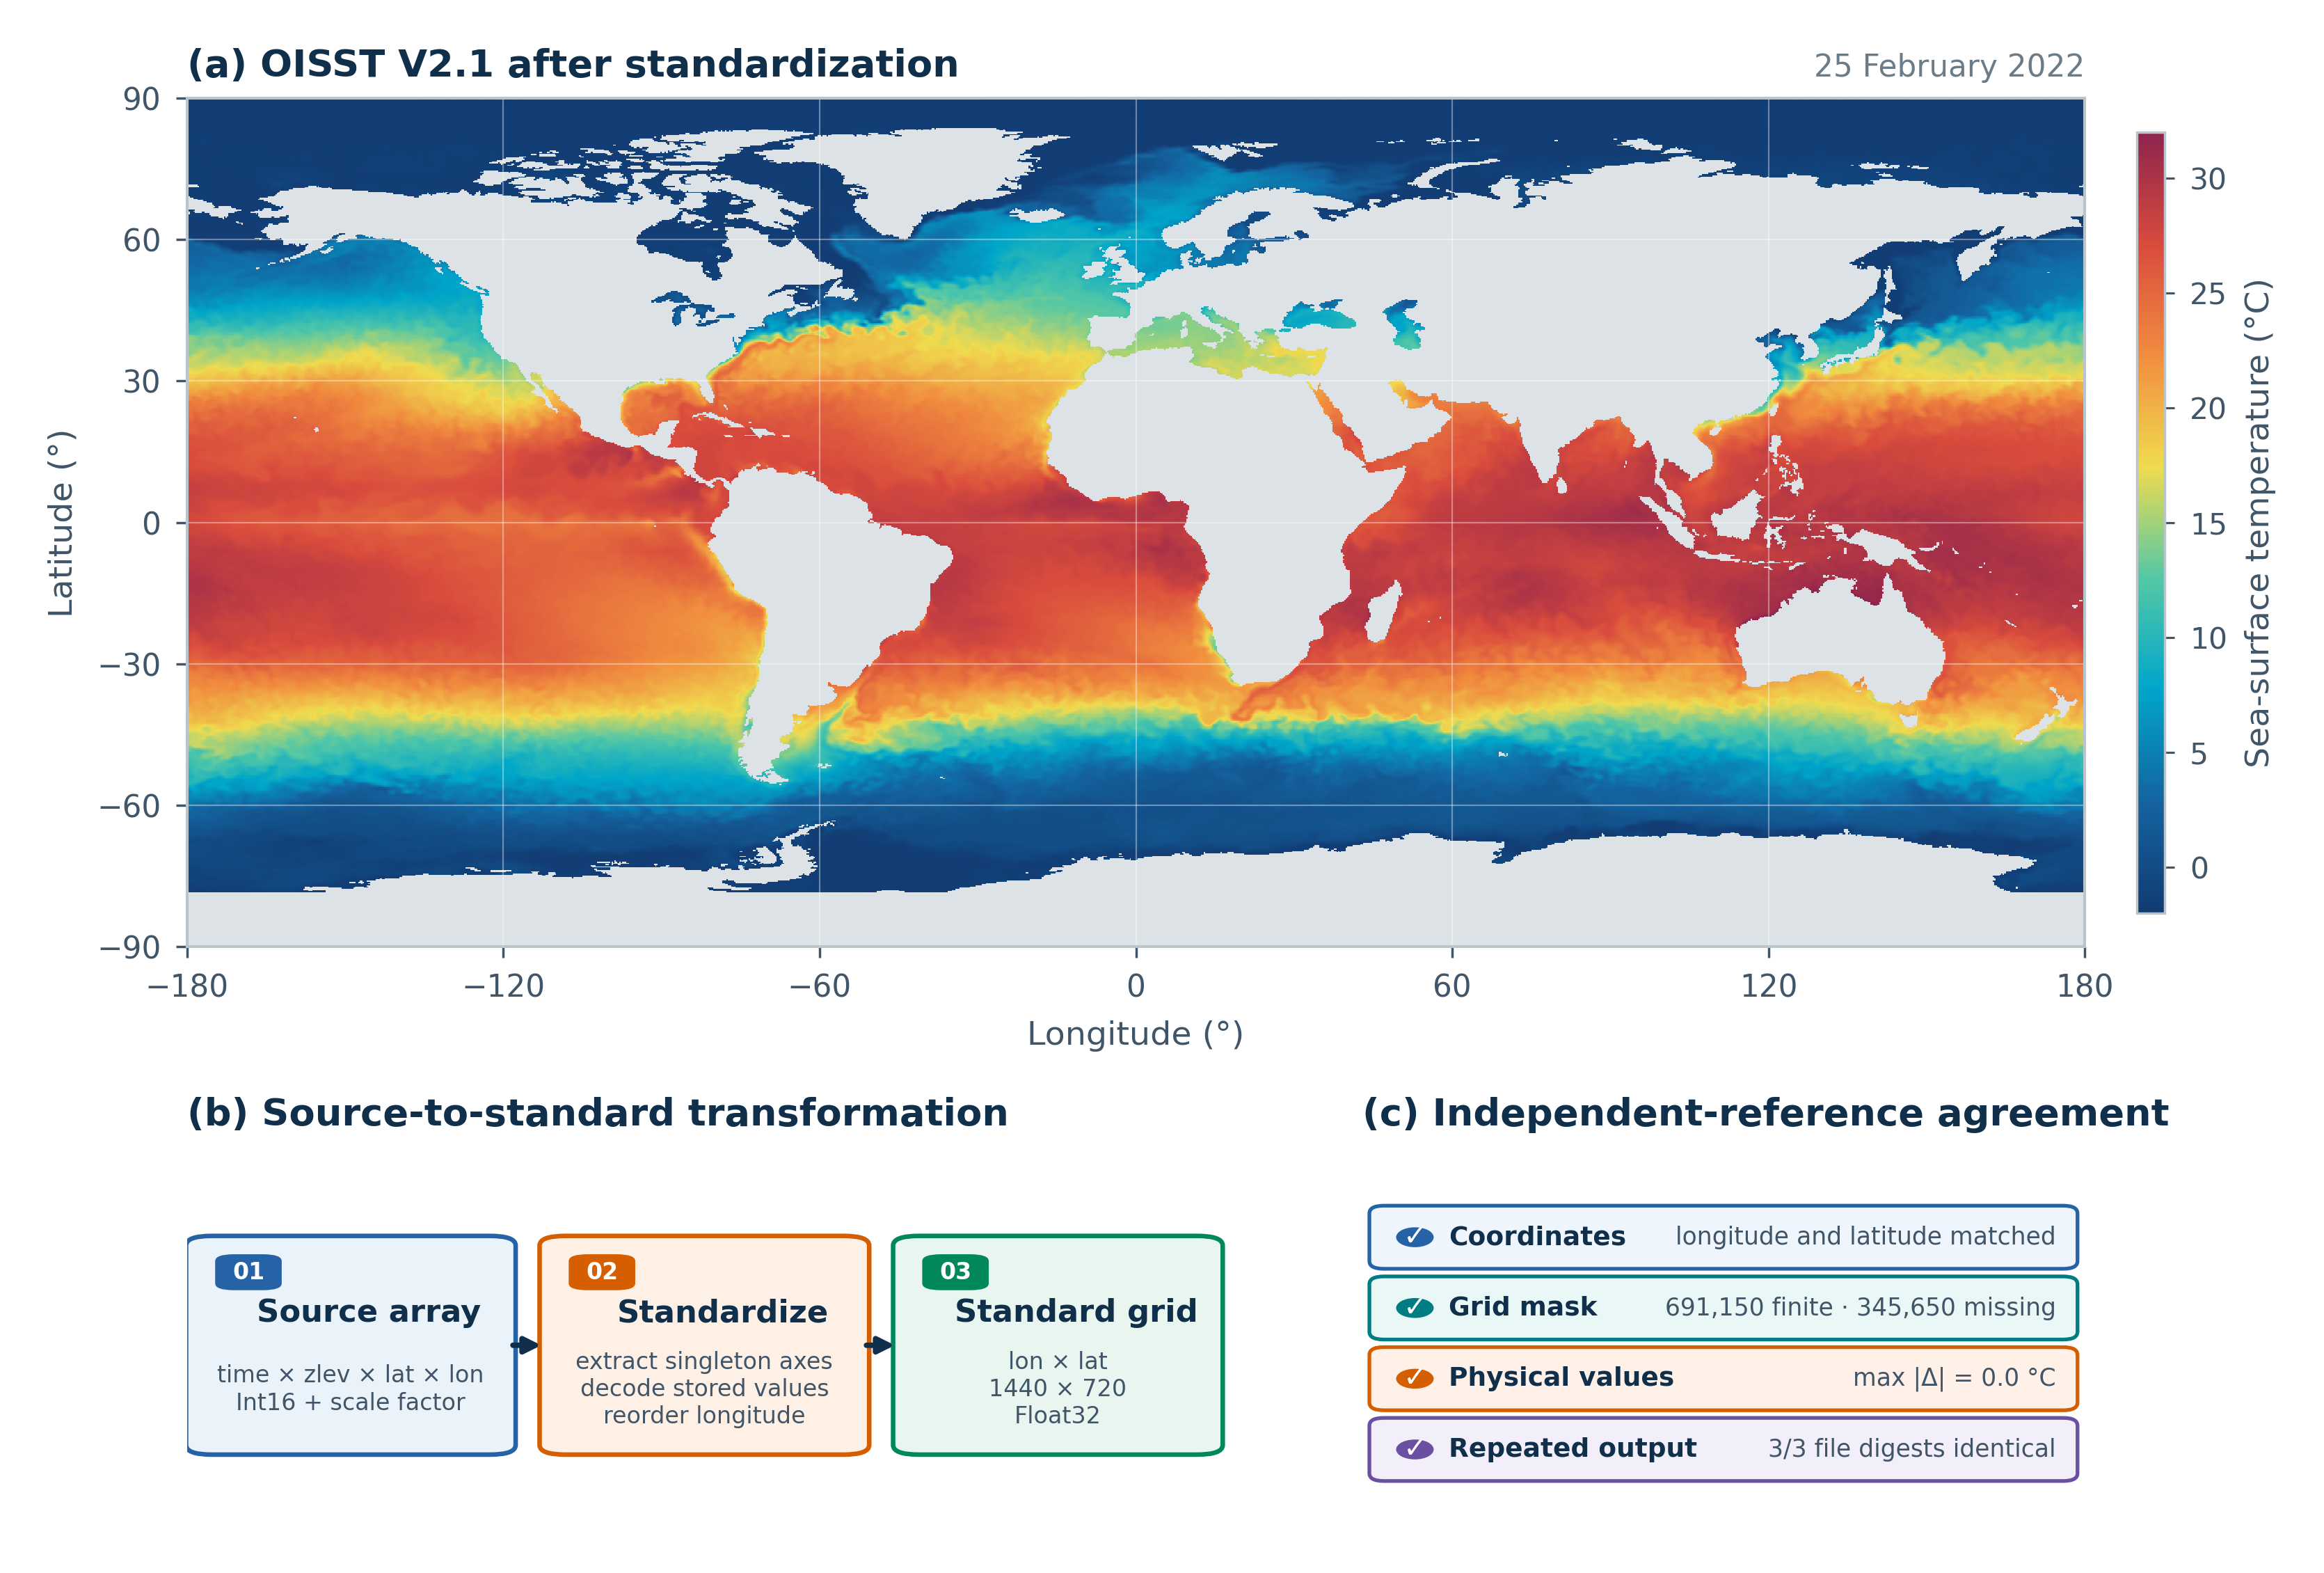
\includegraphics[width=\linewidth,height=0.46\textheight,keepaspectratio]{figures/figure2.png}
\caption*{\textbf{图2 OISST V2.1数据集标准化结果} （a）2022年2月25日全球海表温度标准化数据；（b）从四维源结构、\allowbreak{}存储值解码和经度重排到二维标准网格的转换路径；（c）坐标、\allowbreak{}有效值掩膜、\allowbreak{}物理值及重复生成摘要的独立参考核对。标准化数据为1440\ensuremath{\times}720规则网格，691 150个有效格点及345 650个缺失格点与独立参考掩膜逐点一致，物理值最大绝对差为0，3次生成的文件摘要相同。}
\caption*{\textbf{Fig. 2 Standardization results for the OISST V2.1 dataset.} (a) Global standardized sea-surface temperature on 25 February 2022; (b) the transformation from the four-dimensional source layout through stored-value decoding and longitude reordering to the two-dimensional standard grid; and (c) independent-reference checks of coordinates, the finite-value mask, physical values, and repeated file digests. The 1440 \ensuremath{\times} 720 dataset contains 691,150 finite and 345,650 missing cells that match the independently decoded reference mask point by point, with a maximum absolute physical-value difference of zero and identical file digests across three runs.}
\label{fig:2}
\end{figure}
\subsection{ELEV与LAI的直接NetCDF分发效率}
按照第3.2节的相同输入和测量协议，环境A中直接NetCDF相对外层\nolinkurl{tar.gz}将ELEV和LAI的端到端中位时间分别由40.503和222.297 ms降至20.929和38.100 ms，降幅为48.3\%和82.9\%；环境B中的相应降幅分别为53.6\%和69.2\%（图3）。两个数据文件的传输字节分别增加6.43\%和2.16\%，文件存储占用分别减少约48\%和49\%。80次SHA-256摘要核验结果一致。

两文件均已采用NetCDF内部zlib压缩级别4，对照归档采用gzip级别6。在所测文件和缓存预热条件下，直接NetCDF以较小的传输字节增量减少了解包时间和文件存储占用，缩短了从请求到首次读取数据的路径。

\begin{figure}[!htbp]
\centering
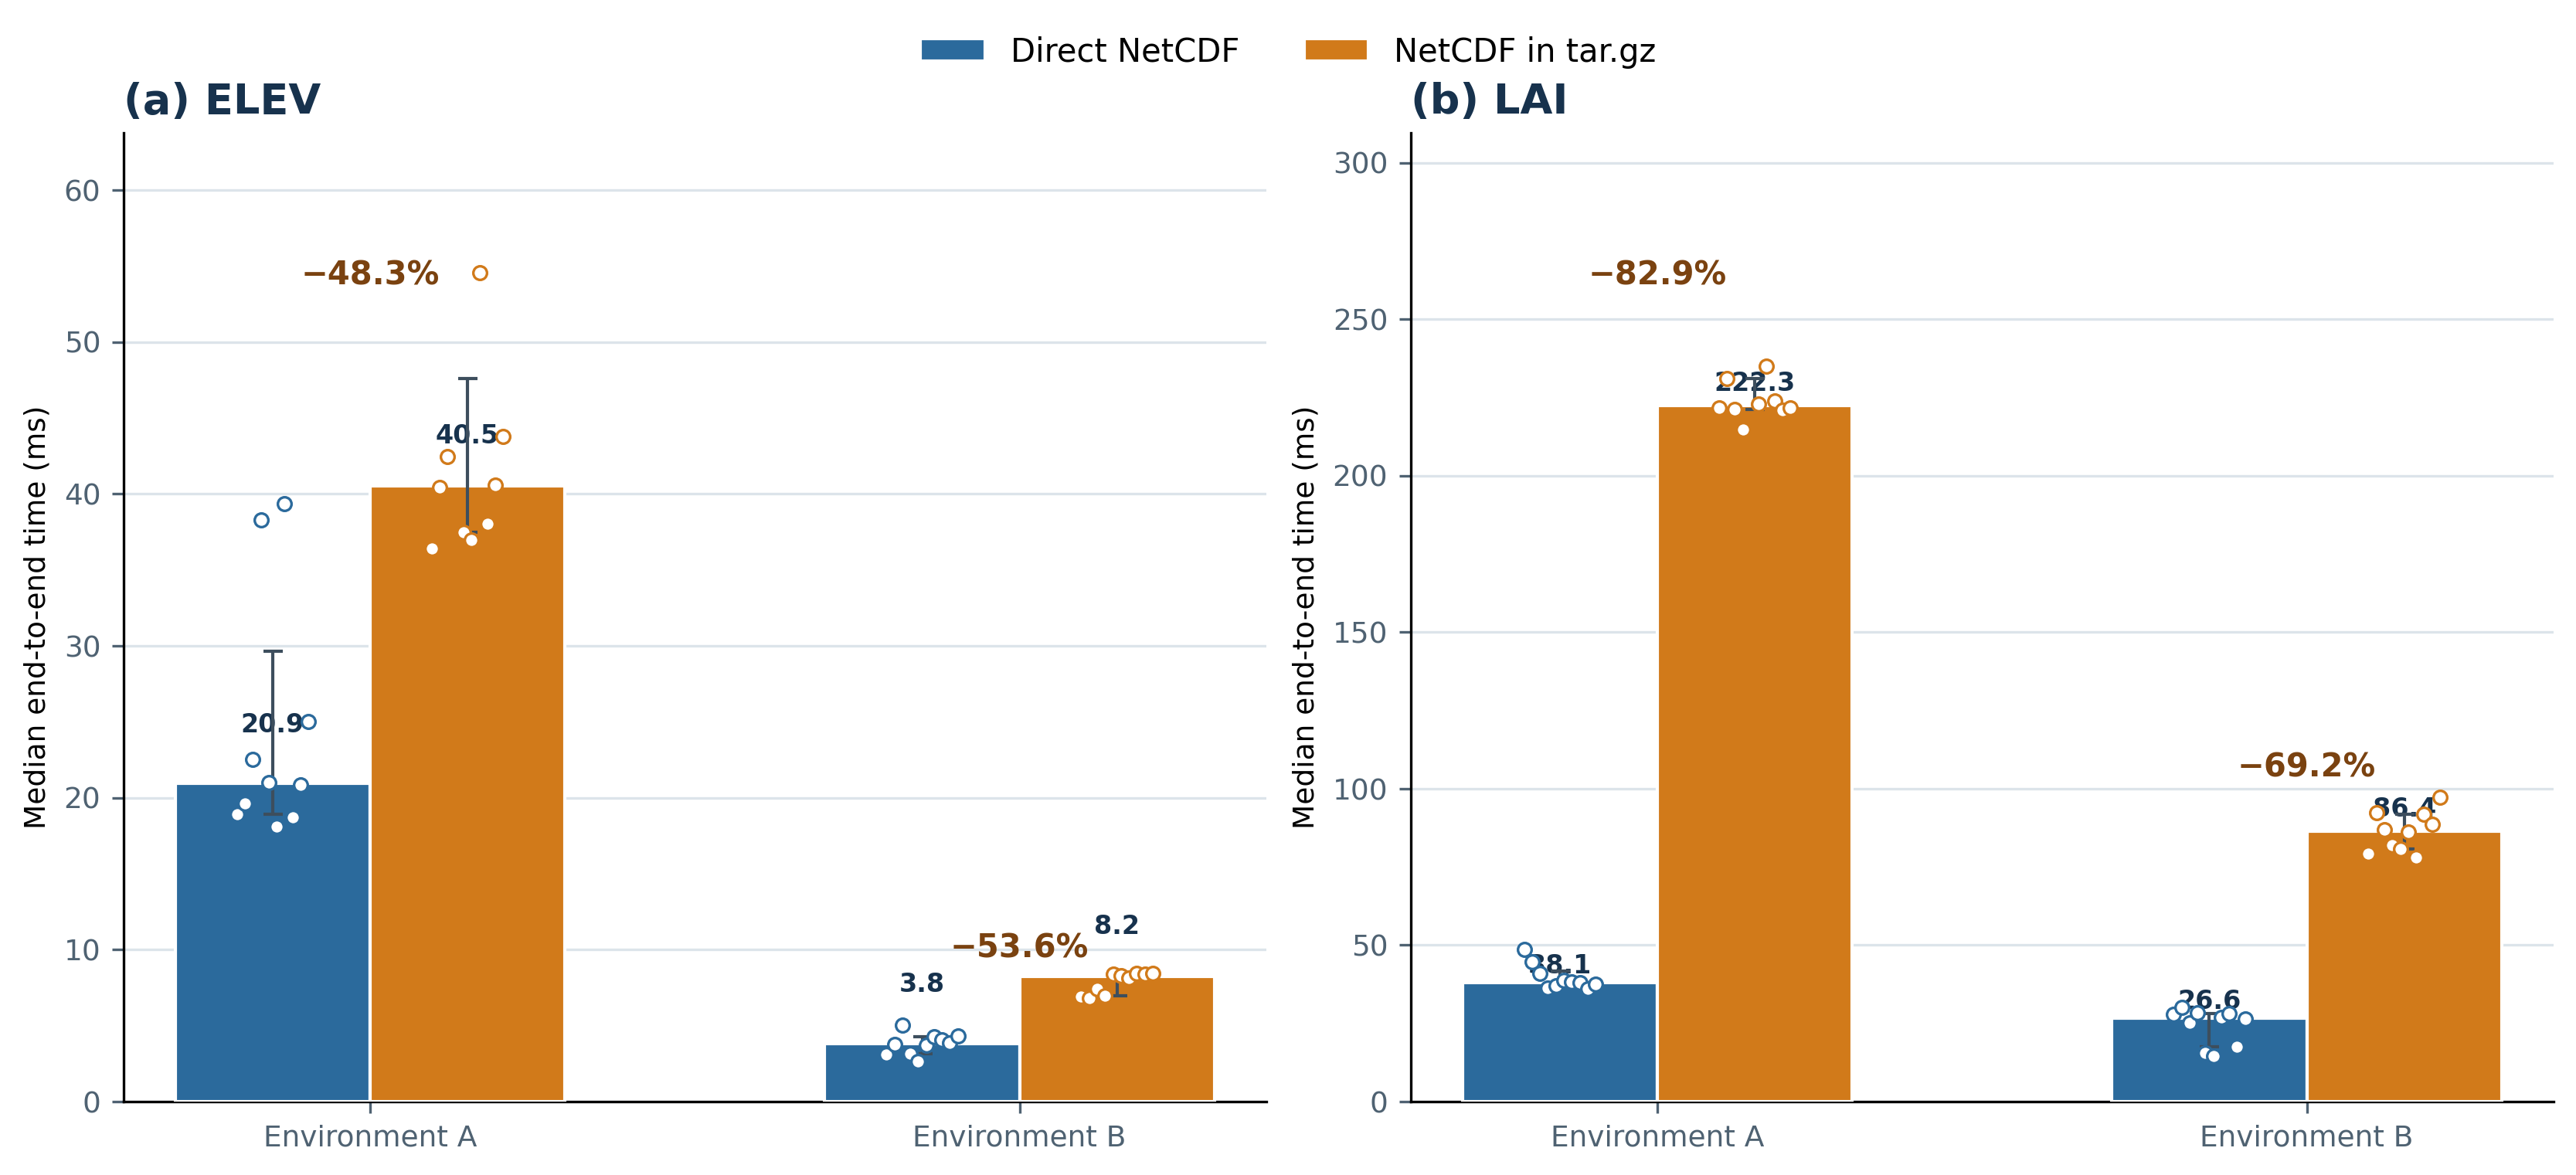
\includegraphics[width=\linewidth,height=0.46\textheight,keepaspectratio]{figures/figure3.png}
\caption*{\textbf{图3 ELEV和LAI数据集采用直接NetCDF与外层tar.gz分发的端到端时间比较} （a）二维高程数据集ELEV；（b）三维叶面积指数数据集LAI。空心圆表示各组合的10次独立测量，柱高为缓存预热后端到端时间中位数，误差线为95\% Bootstrap置信区间；环境A（Windows）和环境B（macOS）采用相同输入文件与测量协议。柱上百分比表示直接NetCDF相对于外层\nolinkurl{tar.gz}归档的中位时间降幅。}
\caption*{\textbf{Fig. 3 End-to-end distribution time for the ELEV and LAI datasets using direct NetCDF and external \nolinkurl{tar.gz} archives.} (a) The two-dimensional ELEV dataset; (b) the three-dimensional LAI dataset. Open circles show the 10 measurements for each combination, bars show median warm-cache end-to-end time, and error bars show 95\% bootstrap confidence intervals. Environment A (Windows) and environment B (macOS) used identical input files and measurement protocols. Percentages above the bars indicate the reduction in median time achieved by direct NetCDF relative to external \nolinkurl{tar.gz} archives.}
\label{fig:3}
\end{figure}
\subsection{目录管理与事务式多镜像分发}
13类受控状态场景在两个独立操作系统环境中各重复5次，镜像回退、\allowbreak{}缓存复用和内容核验结果均符合预设。首选镜像无法访问或未通过内容核验时，程序继续尝试后续镜像；下载失败时，已有正式文件的摘要保持不变。因此，切换镜像无需破坏本地有效缓存，下载异常时科研程序仍可读取已有数据。

公共网络场景中，两个独立环境分别对4个Zenodo标签重复获取3次，共24次下载均与登记字节数和SHA-256一致。下载时间随文件规模呈梯度变化，公共镜像能够向本地科研程序提供内容可核验的数据文件。

中科大校内网场景中，4个数据集分别从FTP和Zenodo重复获取3次，两类镜像各形成12次下载，共24次结果。两类镜像提供的同一数据集均与目录登记的字节数和SHA-256一致，说明机构镜像与公共镜像能够提供内容一致的分发副本。延迟辅助排序与本组实际传输顺序一致；分数据集传输时间与网络记录列于补充材料。

在ERA5降水单位属性由\nolinkurl{mm}修订为\nolinkurl{m}的案例中，独立目录将原逻辑标签\nolinkurl{PPT_ERA5_1X_1H_2020_V1}指向\nolinkurl{V1_R1.nc}，记录修订后的字节数与SHA-256，同时分别保留原V1和R1文件。首次调用获取修订文件并通过完整性核验，后续调用则复用本地缓存。科研程序因此可沿用原标签访问修订数据，而各次试验实际使用的文件可由目录版本与摘要追溯。单位修订依据及模式换算见第4.4节。

\subsection{统一读取与模式输入组织}
不同空间分辨率和时间尺度的14类陆面数据经统一组织，形成2020年US-NR1格点的34个模式字段，包含366日季节序列、\allowbreak{}4个土壤层和17个植物功能型。站点索引映射至40.5°N、\allowbreak{}105.5°W，高程、\allowbreak{}陆地掩膜与叶面积指数的读取结果一致。撒哈拉案例被识别为非植被格点，并按相应陆面状态组织参数，说明同一数据集合能够根据格点状态提供植被与非植被条件下的模式输入。各输入文件的大小、\allowbreak{}来源摘要和SHA-256均通过核验。

8类ERA5气象变量经统一读取，形成US-NR1格点2020年连续的年度逐小时序列。各源变量均为360\ensuremath{\times}180\ensuremath{\times}8784的经度、\allowbreak{}纬度和逐小时数组，并带有单位属性；站点的每类变量均得到8784个逐小时值，有限值比例为100\%，与底层NetCDF读取结果的最大绝对差为0。地方平太阳时偏移为\ensuremath{-}7.0364 h，浮点年积日严格递增且与独立公式逐点一致。时间轴和8类气象变量共9个字段经Emerald接口适配后，组成16个模式驱动字段，完成从格点年度序列到模式所需变量的转换。逐文件大小与字段信息见补充材料S1。

依据ERA5逐小时总降水的变量定义\cite{ref11}，降水输入表示每小时累计的米制水层，标准NetCDF单位属性据此修订为\nolinkurl{m}，数据值保持不变。US-NR1年度累计降水为0.496409 m，即496.409 mm，用于核对数值尺度与量纲。Emerald按水层厚度、\allowbreak{}水密度、\allowbreak{}水的摩尔质量及3600 s累计时段换算为摩尔通量，使数据单位与模式输入一致。完成参数组织、\allowbreak{}时间轴构建和量纲换算后，将真实陆面参数与气象驱动共同用于Emerald初始化和60 s首步计算，大气与土壤关键状态均保持有限值。该年度案例表明，多源标准网格数据能够按明确的空间、\allowbreak{}时间与单位关系形成可用的模式输入。

\subsection{跨操作系统运行一致性与多语言下载结果}
跨操作系统运行中，GriddingMachine和GriddingMachineDatasets的确定性核心流程得到一致的数据结构、\allowbreak{}逐点数值和文件摘要，Emerald合成输入接口的状态均符合预设结果。不同系统能够沿用同一数据约定完成标准化、\allowbreak{}获取和模式输入组织，为科研程序在不同运行环境中使用这些数据提供支持；各系统测试项目与结果见补充材料S5。

Matlab、\allowbreak{}Octave、\allowbreak{}Python、\allowbreak{}R、\allowbreak{}C和Fortran接口通过URL或数据标签获取的文件均与参考内容一致。按标签下载时，首选镜像不可用后能够继续尝试其余镜像；文件大小或摘要不符时，接口返回错误并保留已有文件。这些结果表明，不同语言的科研程序可以共用数据目录和核验规则，自动获取标准化网格数据，无需分别编写下载与内容核验程序。

\section{讨论}
\subsection{相对2022版的更新与科研用途}
2022版GriddingMachine通过统一网格、\allowbreak{}变量和标签提供多源数据访问\cite{ref5}，本研究进一步关注数据持续更新中的重复维护。31组处理实例与OISST结果表明，源数据在维度、\allowbreak{}坐标和数值上的差异可由配置描述，并由通用程序处理；ELEV重复处理结果则表明，已有标准化数据经过同一流程后仍可保持原值。将处理规则与数据文件一同维护，使新增或更新数据能够复用已有转换程序。镜像调整或文件修订后，可单独更新目录中的分发信息，模式程序继续按标签访问数据。

数据库需要持续更新，既有试验也需要能够复现。ERA5降水修订案例说明，更新目录即可使已有标签指向修订文件；保存各次试验使用的目录、\allowbreak{}文件摘要、\allowbreak{}处理配置和代码版本，则能确定当时使用的数据及其转换过程。标签便于程序持续调用，归档记录保留具体试验的输入，两者共同支持数据更新和试验复现。

\subsection{分发效率与科学数据质量}
ELEV和LAI已经使用NetCDF内部压缩，外层归档带来的额外压缩收益较小，却增加了解包时间，以及归档文件与NetCDF文件同时保存时的存储占用。两个环境中的对照结果表明，直接NetCDF分发仅增加少量传输字节，即可缩短端到端时间并减少获取过程中的存储需求。对于一个标签对应一个文件的数据库，下载完成后即可读取，省去了科研调用前的解包操作。

数据质量检查关注维度、\allowbreak{}坐标、\allowbreak{}物理值、\allowbreak{}单位和缺失值处理是否符合约定，下载完整性核验则确认收到的文件是否与目录记录一致。OISST的独立解码比较和ERA5降水单位修订体现了数值与量纲检查的作用，受控镜像场景和真实网络下载记录则支持对获取内容的核验。两类检查结合后，既能追溯数据如何从源文件转换而来，也能确认科研程序实际读取了哪个文件。

\subsection{从标准网格数据到模式输入}
US-NR1案例表明，统一文件格式之后的关键工作是建立变量之间的空间、\allowbreak{}时间和物理联系。不同分辨率的陆面数据按各自网格提取目标位置的参数，季节参数与ERA5逐时气象按共同年度组织，再由模式适配完成字段和量纲转换。降水等累计量还需结合单位和累计时段换算为模式所需通量，使数据的物理含义与模式计算相衔接。将这些关系纳入统一的数据组织方法，能够减少各模式单独整理参数和气象输入的工作。

其他站点和年份可沿用上述读取与数据组织方法；接入不同模式时，可按其空间、\allowbreak{}时间和变量约定调整配置与适配接口。Julia接口用于组织模式输入，非Julia接口用于在已有科研程序中自动获取文件，研究人员可根据所用语言和计算任务选择调用方式。

\subsection{与相关数据基础设施的关系及扩展方向}
现有数据基础设施各有侧重。地球系统数据立方体着重多变量时空数据的联合分析\cite{ref12}。GriddingMachine侧重共享数据在本地模式中的使用，将标准化、\allowbreak{}读取和模式适配组织为可由科研程序调用的流程，Julia实现便于组合这些处理方法\cite{ref13}。Google Earth Engine提供云端遥感访问与计算\cite{ref4}，ESGF支持分布式气候模式数据发现与访问\cite{ref14}，Pangeo及Pangeo Forge支持云端数据组织和可复用处理配方\cite{ref15,ref16}。本文的OISST和US-NR1案例分别展示了数据转换与本地模式应用：处理结果按统一空间约定保存，多源变量再按时间与量纲关系组合为陆面参数和气象驱动。

数据目录是查找和获取文件的依据。国内地球系统科学数据共享研究强调规范分类和目录建设\cite{ref17}，Pooch提供科研文件获取工具，STAC提供地理空间目录描述规范\cite{ref18,ref19}。本研究在标签对应的条目中同时记录分发地址和文件内容信息，使科研程序在镜像切换或数据修订后仍可使用原有调用方式。镜像获取和修订案例表明，这种组织方式便于本地模式持续使用共享数据；后续可进一步与通用目录规范和数据获取工具衔接。

模式使用多源数据时，还需要保存处理规则及其研究出处。软件引用原则、\allowbreak{}科研软件FAIR原则（FAIR4RS）及数字资源库TRUST原则为软件识别、\allowbreak{}复用与资源库维护提供参考\cite{ref20,ref21,ref22}。本文将数据来源、\allowbreak{}配置和软件版本与处理结果共同归档，以便追溯OISST转换和模式输入组织所用的数据与方法。在扩展数据源配置、\allowbreak{}公共镜像和模式接口时，持续保存这些记录，有助于后续数据维护和科研复用。

\section{结论}
本文针对多源网格数据在转换、\allowbreak{}分发和模式接入中需要重复整理与维护的问题，更新了2022版GriddingMachine。新版通过共享配置记录源数据处理规则，利用独立目录维护标签、\allowbreak{}分发地址和文件完整性信息，并将统一读取的数据进一步组织为陆面参数与气象驱动。同时完善Matlab、\allowbreak{}Octave、\allowbreak{}Python和R对新版数据的自动下载支持，新增C和Fortran支持，使不同编程环境能够通过URL或数据标签获取标准化文件。

受控实例和真实数据案例表明，标准化结果的坐标与物理值均与独立参考一致。直接NetCDF分发减少了解包时间和文件存储占用，缩短了获取至首次读取的时间。FTP—Zenodo镜像所提供的文件与目录登记的摘要一致，数据修订后仍可沿用原标签获取。陆面参数与ERA5逐时数据经组合形成US-NR1模式输入，并完成Emerald初始化和60 s首步计算。

更新后的GriddingMachine使研究人员能够复用已整理的数据及其处理规则，减少不同地球系统模式重复整理和维护数据的工作，为全球网格数据库的持续更新和模式试验提供一致的数据基础。后续将继续扩展数据覆盖范围、\allowbreak{}完善公共镜像登记，并适配更多模式接口。

\section*{数据和代码可用性声明}
GriddingMachine.jl源代码公开于\url{https://github.com/CliMA/GriddingMachine.jl}，数据生产代码公开于\url{https://github.com/jhOo1/GriddingMachineDatasets}，Emerald模式接口环境公开于\url{https://github.com/jhOo1/Emerald-paper}，论文补充材料、\allowbreak{}实验协议、\allowbreak{}脚本和结果公开于\url{https://github.com/jhOo1/GriddingMachine_Reaserach}。研究所用代码版本、\allowbreak{}多语言下载入口及验证记录、\allowbreak{}数据修订信息和实验结果索引见补充材料S8，精确提交与稿件冻结信息由\texttt{论文/投稿版本锁定.toml}统一记录。永久归档与DOI信息随最终归档版本同步发布。

\section*{作者贡献}
姜皓：概念设计、\allowbreak{}方法设计、\allowbreak{}软件、\allowbreak{}数据整理、\allowbreak{}初稿撰写。王玉杰：概念设计、\allowbreak{}软件、\allowbreak{}数据整理、\allowbreak{}研究指导、\allowbreak{}项目管理、\allowbreak{}论文审阅与修改。

\begingroup\singlespacing\begin{thebibliography}{99}\small\setlength{\itemsep}{5pt}
\bibitem{ref1}WILKINSON M D, DUMONTIER M, AALBERSBERG I J, et al. The FAIR Guiding Principles for scientific data management and stewardship[J]. Scientific Data, 2016, 3: 160018. DOI: 10.1038/sdata.2016.18.
\bibitem{ref2}REW R, DAVIS G. NetCDF: An interface for scientific data access[J]. IEEE Computer Graphics and Applications, 1990, 10(4): 76-82. DOI: 10.1109/38.56302.
\bibitem{ref3}CF CONVENTIONS COMMITTEE. CF Metadata Conventions[EB/OL]. [2026-09-26]. \url{https://cfconventions.org/}.
\bibitem{ref4}GORELICK N, HANCHER M, DIXON M, et al. Google Earth Engine: Planetary-scale geospatial analysis for everyone[J]. Remote Sensing of Environment, 2017, 202: 18-27. DOI: 10.1016/j.rse.2017.06.031.
\bibitem{ref5}WANG Y, KÖHLER P, BRAGHIERE R K, et al. GriddingMachine, a database and software for Earth system modeling at global and regional scales[J]. Scientific Data, 2022, 9: 258. DOI: 10.1038/s41597-022-01346-x.
\bibitem{ref6}MEDLYN B E, DUURSMA R A, EAMUS D, et al. Reconciling the optimal and empirical approaches to modelling stomatal conductance[J]. Global Change Biology, 2011, 17(6): 2134-2144. DOI: 10.1111/j.1365-2486.2010.02375.x.
\bibitem{ref7}LIN Y S, MEDLYN B E, DUURSMA R A, et al. Optimal stomatal behaviour around the world[J]. Nature Climate Change, 2015, 5: 459-464. DOI: 10.1038/nclimate2550.
\bibitem{ref8}WALKER A P, BECKERMAN A P, GU L, et al. The relationship of leaf photosynthetic traits—Vcmax and Jmax—to leaf nitrogen, leaf phosphorus, and specific leaf area: A meta-analysis and modeling study[J]. Ecology and Evolution, 2014, 4(16): 3218-3235. DOI: 10.1002/ece3.1173.
\bibitem{ref9}HERSBACH H, BELL B, BERRISFORD P, et al. The ERA5 global reanalysis[J]. Quarterly Journal of the Royal Meteorological Society, 2020, 146(730): 1999-2049. DOI: 10.1002/qj.3803.
\bibitem{ref10}HUANG B, LIU C, BANZON V, et al. Improvements of the Daily Optimum Interpolation Sea Surface Temperature (DOISST) Version 2.1[J]. Journal of Climate, 2021, 34(8): 2923-2939. DOI: 10.1175/JCLI-D-20-0166.1.
\bibitem{ref11}COPERNICUS CLIMATE CHANGE SERVICE. Conversion table for accumulated variables (total precipitation/fluxes)[EB/OL]. [2026-09-26]. \url{https://confluence.ecmwf.int/pages/viewpage.action?pageId=197702790}.
\bibitem{ref12}MAHECHA M D, GANS F, BRANDT G, et al. Earth system data cubes unravel global multivariate dynamics[J]. Earth System Dynamics, 2020, 11: 201-234. DOI: 10.5194/esd-11-201-2020.
\bibitem{ref13}BEZANSON J, EDELMAN A, KARPINSKI S, et al. Julia: A fresh approach to numerical computing[J]. SIAM Review, 2017, 59(1): 65-98. DOI: 10.1137/141000671.
\bibitem{ref14}CINQUINI L, CRICHTON D, MATTMANN C, et al. The Earth System Grid Federation: An open infrastructure for access to distributed geospatial data[J]. Future Generation Computer Systems, 2014, 36: 400-417. DOI: 10.1016/j.future.2013.07.002.
\bibitem{ref15}ABERNATHEY R P, AUGSPURGER T, BANIHIRWE A, et al. Cloud-native repositories for big scientific data[J]. Computing in Science \& Engineering, 2021, 23(2): 26-35. DOI: 10.1109/MCSE.2021.3059437.
\bibitem{ref16}STERN C, ABERNATHEY R, HAMMAN J, et al. Pangeo Forge: Crowdsourcing analysis-ready, cloud optimized data production[J]. Frontiers in Climate, 2022, 3: 782909. DOI: 10.3389/fclim.2021.782909.
\bibitem{ref17}王卷乐, 林海, 冉盈盈, 等. 面向数据共享的地球系统科学数据分类探讨[J]. 地球科学进展, 2014, 29(2): 265-274. DOI: 10.11867/j.issn.1001-8166.2014.02.0265. [WANG Juanle, LIN Hai, RAN Yingying, et al. A study of Earth System Science data classification for data sharing[J]. Advances in Earth Science, 2014, 29(2): 265-274.]
\bibitem{ref18}UIEDA L, SOLER S R, RAMPIN R, et al. Pooch: A friend to fetch your data files[J]. Journal of Open Source Software, 2020, 5(45): 1943. DOI: 10.21105/joss.01943.
\bibitem{ref19}OPEN GEOSPATIAL CONSORTIUM. SpatioTemporal Asset Catalog (STAC) Community Standard, Version 1.1.0[S/OL]. OGC 25-004, 2025 [2026-09-26]. \url{https://www.ogc.org/standards/stac/}.
\bibitem{ref20}SMITH A M, KATZ D S, NIEMEYER K E, et al. Software citation principles[J]. PeerJ Computer Science, 2016, 2: e86. DOI: 10.7717/peerj-cs.86.
\bibitem{ref21}BARKER M, CHUE HONG N P, KATZ D S, et al. Introducing the FAIR Principles for research software[J]. Scientific Data, 2022, 9: 622. DOI: 10.1038/s41597-022-01710-x.
\bibitem{ref22}LIN D, CRABTREE J, DILLO I, et al. The TRUST Principles for digital repositories[J]. Scientific Data, 2020, 7: 144. DOI: 10.1038/s41597-020-0486-7.
\end{thebibliography}\endgroup
\end{CJK}
\end{document}
